\subsubsubsubsection{Stretch Sign Decorator}
\begin{figure}[h]
\centering
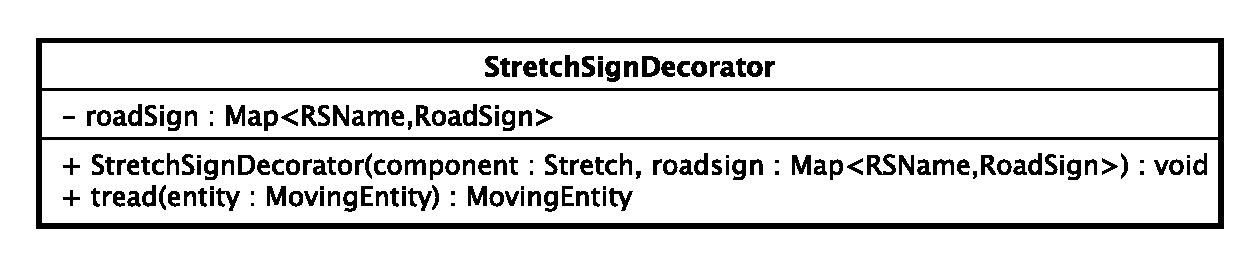
\includegraphics[scale=0.6,keepaspectratio]{images/solution/stretch_sign_decorator.eps}
\caption{App::Reactive::StretchSignDecorator}
\label{fig:sd-app-stretch_sign_decorator}
\end{figure}
\FloatBarrier
\begin{itemize}
  \item \textbf{Description} \\
    It represents a decorator which adds road signs' behaviour on the top of the
    standard stretch behaviour. 
  \item \textbf{Attribute}
  \begin{itemize}
    \item \texttt{- roadSign: Map<RSName, RoadSign>} \\
The map of road signs to consider during the decoration.
  \end{itemize}
  \item \textbf{Operation}
   \begin{itemize} 
   \item \texttt{+ StretchSignDecorator(component: Stretch, roadSign: Map<RSName, RoadSign>)} \\
Creates a stretch sign decorator with a specific stretch to decorate and a map of road signs to apply as decorations.
    \item \texttt{+ tread(entity: MovingEntity)} \\
Decorates the standard behaviour of the stretch with road signs.  
  \end{itemize}
\end{itemize}
